% Author: Izaak Neutelings (Februari, 2020)
% !TEX root = /home/eb/Dropbox/CPGE/Physique/Cours/[5]Electromg/[2]ExElec/Figures/capacitors.tex
\documentclass[border=3pt,tikz]{standalone}
\usepackage{amsmath} % for \dfrac
\usepackage{bm}
\usepackage{physics}
\usepackage{tikz,pgfplots}
\usetikzlibrary{angles,quotes} % for pic (angle labels)
\usetikzlibrary{decorations.markings}
\usetikzlibrary{calc}
\tikzset{>=latex} % for LaTeX arrow head

\usepackage{xcolor}
\colorlet{Ecol}{orange!90!black}
\colorlet{EcolFL}{orange!90!black}
\colorlet{veccol}{green!45!black}
\colorlet{EFcol}{red!60!black}
\colorlet{pluscol}{red!60!black}
\colorlet{minuscol}{blue!60!black}
\tikzstyle{anode}=[top color=red!20,bottom color=red!50,shading angle=20]
\tikzstyle{cathode}=[top color=blue!20,bottom color=blue!40,shading angle=20]
\tikzstyle{charge+}=[very thin,top color=red!80,bottom color=red!80!black,shading angle=-5]
\tikzstyle{charge-}=[very thin,top color=blue!50,bottom color=blue!70!white!90!black,shading angle=10]
\tikzstyle{vector}=[->,thick,veccol]
\tikzstyle{normalvec}=[->,thick,blue!80!black!80]
\tikzstyle{Cstyle}=[very thick,orange!90!black]
\tikzstyle{EField}=[->,thick,Ecol]
\tikzstyle{EField dashed}=[dashed,Ecol,line width=0.6]
\tikzset{
  EFieldLine/.style={thick,EcolFL,decoration={markings,
                     mark=at position #1 with {\arrow{latex}}},
                     postaction={decorate}},
  EFieldLine/.default=0.5}
\tikzstyle{measure}=[fill=white,midway,outer sep=2]

\def\dpa{0.28}
\def\dba{0.14}
\def\dipole#1#2{
  \begin{scope}[shift={(#1)},rotate=#2]
    \draw[charge-] (-\dpa,0) to[out=90,in=180] (0,\dba) -- (0,-\dba) to[out=180,in=-90] cycle;
    \draw[charge+] ( \dpa,0) to[out=90,in=  0] (0,\dba) -- (0,-\dba) to[out=  0,in=-90] cycle;
    \node[scale=0.7] at (-\dpa/2,0) {$-$};
    \node[scale=0.7] at ( \dpa/2,0) {$+$};
  \end{scope}
}

\begin{document}


% CAPACITOR 3D
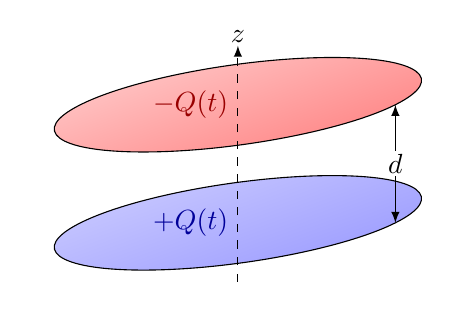
\begin{tikzpicture}[x={(1cm,0)},y={(0.6cm,0.3cm)},z={(0,1cm)}]
  \def\H{1.5}
  \def\W{4}
  \def\L{2}
  \def\Nx{5}
  \def\Ny{10}
  \draw[cathode]
    (0,0,0) circle(\L);
  \draw[anode]
    (0,0,\H) circle(\L);
  % \foreach \i [evaluate={\r=\i*\L/\Nx;}] in {1,...,\Nx}{
  %   \foreach \j [evaluate={\t=\j*360/\Ny;}] in {1,...,\Ny}{
  %     \node[minuscol,scale=0.8] at (\t:\r) {$-$};
  %     \node[pluscol,scale=0.8] at (\t:\r) {$+$};
  %   }
  % }
  \node[minuscol,left] at (0,0,0) {$+Q(t)$};
  \node[pluscol,left] at (0,0,\H) {$-Q(t)$};
  % \node[left=2,above left=1] at (\L,\W,\H) {$A$};
  \draw[dashed,->] (0,0,-0.5*\H) -- (0,0,1.5*\H) node[above,inner sep=1pt] {$z$};
  \draw[<->] (\L,0,0) -- (\L,0,\H) node[measure,inner sep=1pt] {$d$};
\end{tikzpicture}
\end{document}
